\section{Альтернативный алгоритм распределения заказов}

	DESC:  При поступлении заказа по одному из каналов сервер формирует очередь из водителей и обрабатывает ее, в результате заказ будет взят на выполнение одним из них.

	Альтернативный алгоритм обработки заказов находится в Приложении 1.

	Диаграмма:

	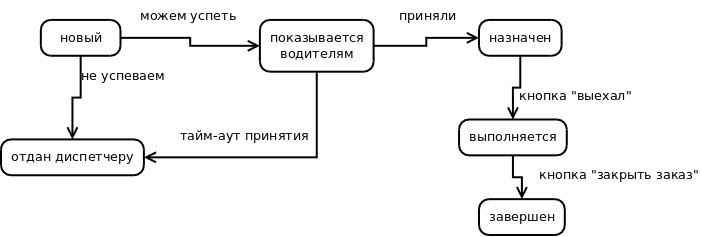
\includegraphics[width=\textwidth]{images/appendices/alt_alg}

	\subsection{Фильтрация водителей}

		DESC: Сервер выбирает из базы данных водителей под заказ.

		\subsubsection{Стандартная фильтрация водителей}

			Требования:

			\begin{enumerate}
				\item{Сервер проверяет тип заказа.}

				\item{Сервер выбирает водителей, которые удовлетворяют следующим условиям: \begin{enumerate}[label*=\arabic*.] \item{Они удовлетворяют параметрам заказа.} \item{В их диапазоны попадает начальная точка заказа, т.е. они либо имеют статус “свободен”, либо у них включен робот “цепочка” или “поиск по адресу”.} \end{enumerate}}

				\item{Для каждого из этих водителей сервер с помощью Яндекс.Пробок вычисляет \textit{расчетное время подачи машины}: \begin{enumerate}[label*=\arabic*.] \item{Для свободных водителей это просто время, необходимое, чтобы доехать до клиента с учетом дорожной обстановки.} \item{Для водителей с роботом “цепочка” - это расчетное время до завершения текущего заказа плюс время, чтобы доехать до клиента.} \item{Для водителей с роботом “поиск по адресу” - это время, оставшееся до указанного в настройках робота, плюс время, чтобы доехать до клиента от указанного адреса.} \item{Ко всем трем вышеперечисленным пунктам добавляется “Страховочное время” установленное владельцем.} \end{enumerate}}

				\item{Водители, у которых расчетное время подачи машины превышает время, оставшееся до заявленного клиентом, исключаются из дальнейшего рассмотрения.}

				\item{Также из дальнейшего рассмотрения исключаются те водители, которым выполнение данного заказа помешает выполнить один из закрепленных за ними ранее предварительных заказов. Для этого проверяется, что после выполнения данного, нового, заказа водитель будет иметь достаточно времени, чтобы вовремя подать машину на полученный ранее предварительный заказ.}

				\item{Если после фильтрации не осталось ни одного водителя, то заказ предается компании-партнеру, но только в том случае если параметры заказа соответствуют условиям передачи заказа партнерам выставленными владельцем.}
			\end{enumerate}

		\subsubsection{Фильтрация водителей для заказов от Яндекс}

			Требования:

			\begin{enumerate}
				\item{Сервер выбирает водителей, которые удовлетворяют следующим условиям: \begin{enumerate}[label*=\arabic*.] \item{Они удовлетворяют параметрам заказа.} \item{В их диапазоны попадает начальная точка заказа.} \end{enumerate}}
			\end{enumerate}

		\subsubsection{Диапазоны в фильтрации}

			Требования:

			\begin{enumerate}
				\item{Согласно километражу выставленным водителем, сервер вычисляет диапазон принятия заказа относительно местоположения водителя.}

				\item{Если водитель не в цепочке то его диапазон принятия заказа равен радиусу.}

				\item{Если водитель в цепочке и у него нет следующего заказа, то его диапазон d = (r -c)/2, при условии c<r где r - максимальный радиус взятия заказа установленный водителем (километраж), а c - расстояние между местоположением водителя и конечной точкой текущего заказа водителя.}

				\item{Если c > r, то d =0}
			\end{enumerate}

	\subsection{Построение очереди для заказов от Диспетчерской и партнеров}

		DESC: Сервер выстраивает очередь из водителей которые прошли фильтрацию заказа(SRV-9.1).

		\subsubsection{Построение очереди для срочных заказов от Диспетчерской и партнеров}

			Требования:

			\begin{enumerate}
				\item{Сервер конвертирует расчетное время подачи машины в условные единицы сортирует водителей по убыванию этих значений.}

				\item{Сервер отправляет запрос в базу данных о количестве выполненных заказов за N часов для всех водителей в списке и прибавляет каждому из водителей N условных единиц  за каждый выполненный заказ.}

				\item{Если водитель из списка прошел фильтрацию по параметрам роботов “Поиск по адресу” и “Хочу домой”, то ему прибавляется N условных единиц.}

				\item{Если водитель из списка прошел фильтрацию по предварительным заказам, то сервер вычисляет разницу между временем выполнения потенциально заказа и предварительного, и: \begin{enumerate}[label*=\arabic*.] \item{Если эта разница ниже чем интервал установленный владельцем, то сервер отбавляет N условных единиц данному водителю.} \item{Если эта разница в пределах интервала установленный владельцем, то сервер прибавляет N условных единиц данному водителю.} \item{Если эта разница превышает интервал установленный владельцем то сервер никак не изменяет значение.} \end{enumerate}}

				\item{Сервер показывает заказ всем водителям в очереди с задержкой пропорциональной разнице между расчетными условными единицами между водителями.}

				\item{В случае если водитель прислал запрос на подтверждение заказа или у водителя в очереди был включен робот, сервер закрепляет за ним заказ и учитывает его при фильтрации на новые заказы.}

				\item{Если за фиксированное время, выставленное владельцем, ни один из водителей не подобрал заказ, то заказ становится видимым всем, и если в течении n минут никто не подобрал заказ, то он передается партнерам.}
			\end{enumerate}

		\subsubsection{Построение очереди для предварительных заказов от Диспетчерской}

			Требования:

			\begin{enumerate}
				\item{Если поступил предварительный заказ, то он сохраняется в базе данных.}

				\item{Заказ показывается за N минут до времени подачи.}

				\item{Для заказа строится очередь по алгоритму из SRV-9.2.1}

				\item{Если заказ с дополнительными параметрами (детское кресло, кредитная карта и т.д.), то к N минутам прибавляется время, устанавливаемое владельцем, каждого из параметров. В этом случае сервер показывает заказ всем водителям подходящим по параметрам. Как только проходит контрольное время сервер выстраивает очередь на заказ(см. пункт 3).}

				\item{В случае если водитель прислал запрос на подтверждение заказа или у водителя в очереди был включен робот, сервер закрепляет за ним заказ и учитывает его при фильтрации на новые заказы.}

				\item{Если за фиксированное время, выставленное владельцем, ни один из водителей не подобрал заказ, то заказ становится видимым всем, и если в течении n минут никто не подобрал заказ, то он передается партнерам.}
			\end{enumerate}

		\subsubsection{Построение очереди для портовых заказов от Диспетчерской}

			DESC: Владелец очерчивает вручную на карте диапазон координат с границами порта. Сервер выстраивает две очереди на портовые заказы - приоритетная и обычная.

			Требования:

			\begin{enumerate}
				\item{Если водитель приехал в порт с заказом, сервер ставит его в конец приоритетной очереди, если без - обычной.}

				\item{При поступлении портового заказа типа “Встреча”, сервер отправляет первому водителю в приоритетной очереди запрос с информацией о заказе. }

				\item{Помимо информации о заказе сервер передает водителю его номер в очереди.}

				\item{Далее сервер передает запросы о заказе остальным водителям в приоритетной очереди с задержкой в N секунд, затем переключается на обычную очередь где с такой же задержкой передает запросы.}

				\item{В случае если никто не взял заказ, за определенный промежуток времени до времени подачи, заказ показывается всем водителям.}
			\end{enumerate}

	\subsection{Подбор водителей для заказов от Яндекс.Такси}

		DESC: Сервер принимает срочные и не срочные заказы от Яндекс.Такси.

		Требования:

		\begin{enumerate}
			\item{Если заказ срочный, то Яндекс.Такси присылает список водителей.}

			\item{Если заказ не срочный, то сервер выбирает из базы данных водителей соответствующих критериям указанным в SRV-9.2 и составляет свой список водителей.}

			\item{Заказ делается видимым для всех водителей из списка.}

			\item{Сервер проверяет список на наличие водителей с включенными роботами, и если один или несколько из выбранных сервером водителей проходит проверку, то от лица каждого из этих водителей на сервер Яндекс.Такси отправляется запрос на закрепление заказа за ними.}

			\item{Если один из водителей без включенного робота готов принять заказ, сервер отсылает Яндексу запрос на подтверждение. Если при этом приходит ответ, что заказ уже ушел в другую службу такси - заказ удаляется из списка заказов.}

			\item{Если Яндекс.Такси присылает подтверждение о закреплении заказа за одним из водителей, то ему отсылается сообщение о новом заказе.}

			\item{Если от Яндекса приходит оповещения об отмене заказа (ушел к другой службе, отменен клиентом) - заказ удаляется из списка заказов.}
		\end{enumerate}

	\subsection{Приоритеты}

		DESC: Если водитель стоит сразу в нескольких очередях, сервер подбирает водителю заказ оптимально используя ресурсы Службы-Такси. Это требование опциональное, владелец может использовать стандартный вариант с приоритетом по времени.

		Требования:

		\begin{enumerate}
			\item{Заказ поступивший от Яндекс.Такси имеет большой приоритет чем заказы поступившие из остальных каналов.}

			\item{Сервер выбирает нижестоящих по списку водителей в двух или более очередях, по отношению к текущему водителю.}

			\item{Сервер выбирает наименьшую по количеству водителей очередь, из тех в которых состоит водитель, и добавляет N условных единиц к расчетным единицам для этого водителя в данной очереди.}

			\item{Сервер выбирает наименьшую по количеству водителей с роботами очередь, из тех в которых состоит водитель, и добавляет N условных единиц к расчетным единицам для этого водителя в данной очереди.}

			\item{Сервер выбирает наименьшую по количеству состоящих в других очередях водителей очередь, из тех в которых состоит водитель, и добавляет N условных единиц к расчетным единицам для этого водителя в данной очереди.}

			\item{Сервер выбирает наименьшую по количеству водителей с роботами (состоящих в других очередях) очередь, из тех в которых состоит водитель, и добавляет N условных единиц к расчетным единицам для этого водителя в данной очереди.}
		\end{enumerate}


